\documentclass{article}
\usepackage{neurips_2024}
\usepackage[utf8]{inputenc}
\usepackage[T1]{fontenc}
\usepackage{hyperref}
\usepackage{url}
\usepackage{booktabs}
\usepackage{amsfonts}
% \usepackage{nicefrac}  % not installed
% \usepackage{microtype} % not installed
\usepackage{graphicx}
\usepackage{xcolor}
\usepackage{tikz}
\usetikzlibrary{positioning, arrows.meta, shapes.geometric, fit, calc}

\title{RestReflect: A Privacy-First Voice Companion\\for Therapeutic Reflection Using Local AI}

\author{
  Eugenio Rivera Ramos \\
  \texttt{42euge@gmail.com}
}

\begin{document}

\maketitle

\begin{abstract}
Mainstream AI voice assistants optimize for task completion speed---detecting silence, assuming the user is done, and generating an answer as fast as possible. This paradigm fails for therapeutic conversation, where silence is intentional, reflection precedes advice, and privacy determines what users are willing to say. We present RestReflect, a fully local voice companion for therapeutic reflection that runs entirely on Apple Silicon with no cloud dependencies. The system's central feature is \emph{Reflect Mode}---a real-time pipeline that listens to the user via streaming speech-to-text, concurrently analyzes emotional content and conversational themes through a local LLM, and mirrors back what the user said as synthesized speech, implementing reflective listening from motivational interviewing (MI). Reflect Mode is supported by a multi-signal turn-taking engine that treats silence as therapeutic space (4--16\,s adaptive thresholds vs.\ the 0.3--0.5\,s industry standard), a real-time emotional activation tracker that adjusts system \emph{behavior}---not just tone---based on pitch, energy, and vocal tension, and an ambient particle canvas whose visual state (ambient drift, spectrum-driven disturbance, gravitational collapse) communicates whether the system is listening, responding, or preparing a deep reflection---without breaking silence. All components---Whisper STT, Gemma~4 LLM, Kokoro TTS, Silero VAD, and a custom activation tracker---run on-device, ensuring that therapy-sensitive audio never leaves the user's machine.
\end{abstract}

%----------------------------------------------------------------------
\section{Introduction}
%----------------------------------------------------------------------

There are things people cannot talk about---not to friends, not to family, not to anyone. The weight of carrying the unspeakable is itself a source of suffering. Traditional therapy, while effective, is inaccessible for most: constrained by cost, availability, and stigma. Even when accessible, some disclosures feel too raw to voice to another human.

AI-assisted mental health tools have emerged to fill this gap. Woebot~\citep{fitzpatrick2017woebot}, Wysa~\citep{inkster2018wysa}, and similar platforms deliver CBT-based interventions through text chatbots, and frontier voice agents like ChatGPT Advanced Voice Mode and Gemini Live now offer real-time spoken conversation with impressive latency. However, all existing approaches share a critical limitation: they require users to send their most sensitive thoughts to remote servers. This creates a \emph{privacy paradox}---the population most in need of AI-assisted reflection (those dealing with trauma, shame, stigma, or trust issues) is precisely the population least likely to trust cloud services with their innermost thoughts.

Beyond privacy, mainstream voice agents are architecturally misaligned with therapeutic conversation. They detect silence for 300--500\,ms, assume the user has finished, and race to generate a response. No commercial voice agent produces reflective restatements before answering, holds therapeutic silence, or adjusts its \emph{behavior} based on the user's emotional state. The optimization target is response speed \emph{at every moment}---these systems never choose not to respond. RestReflect separates the problem: \emph{when} to speak is governed by therapeutic judgment (default: silence), but \emph{once the system decides to speak}, time to first speech is optimized aggressively.

RestReflect addresses both problems simultaneously. It is a privacy-first reflection and mindfulness application where the entire AI pipeline runs on the user's device. It implements a therapeutic voice companion grounded in CBT and motivational interviewing~\citep{miller2013motivational}, with a turn-taking engine that defaults to silence, an emotional activation tracker that adjusts system behavior based on audio features, and an ambient particle canvas that provides visual feedback without demanding attention.

\textbf{Research question.} Can a fully local, privacy-preserving AI system provide meaningful therapeutic reflection that users would trust with thoughts they would not share with any cloud service---while maintaining clinical safety and grounding?

%----------------------------------------------------------------------
\section{Related Work}
%----------------------------------------------------------------------

\paragraph{AI-assisted mental health.} Digital interventions have progressed from \citet{weizenbaum1966eliza}'s ELIZA to evidence-based chatbots. Woebot~\citep{fitzpatrick2017woebot} delivers structured CBT exercises and has received FDA breakthrough device designation. Wysa~\citep{inkster2018wysa} combines CBT, DBT, and meditation with clinician oversight. All existing tools are cloud-hosted. RestReflect is, to our knowledge, the first fully local, privacy-by-design therapeutic AI system.

\paragraph{Voice agents.} Mainstream voice agents share five commitments that make them unsuitable for therapeutic use: (1)~VAD-gated turn-taking with 300--500\,ms silence thresholds; (2)~answer-first response with no reflective restatements; (3)~cloud inference for all audio processing; (4)~speed-optimized latency applied indiscriminately---ChatGPT Realtime targets 250--800\,ms first-token audio regardless of whether a response is appropriate; and (5)~passive affect detection that adjusts response \emph{tone} but never response \emph{behavior}.

\paragraph{Reflective listening.} Reflective listening originates from \citet{rogers1957necessary}'s person-centered therapy and is foundational in Motivational Interviewing~\citep{miller2013motivational}. \citet{magill2018meta} meta-analyzed 21~MI studies finding therapist reflective listening correlated with client change talk ($r = .55$, $p < .001$). \citet{kumar2024gpt4} showed GPT-4 generates complex backward-looking reflections with 88\% clinician-rated acceptability.

\paragraph{Affect labeling.} \citet{lieberman2007putting} showed via fMRI that verbally labeling an emotion decreases amygdala activation and engages prefrontal regulation circuits. \citet{plutchik1980general}'s wheel of emotions provides a structured taxonomy that scaffolds this labeling process.

%----------------------------------------------------------------------
\section{System Architecture}
%----------------------------------------------------------------------

RestReflect is a modular system with a thin orchestrator delegating to specialized components (Figure~\ref{fig:arch}).

\begin{figure}[h]
\centering
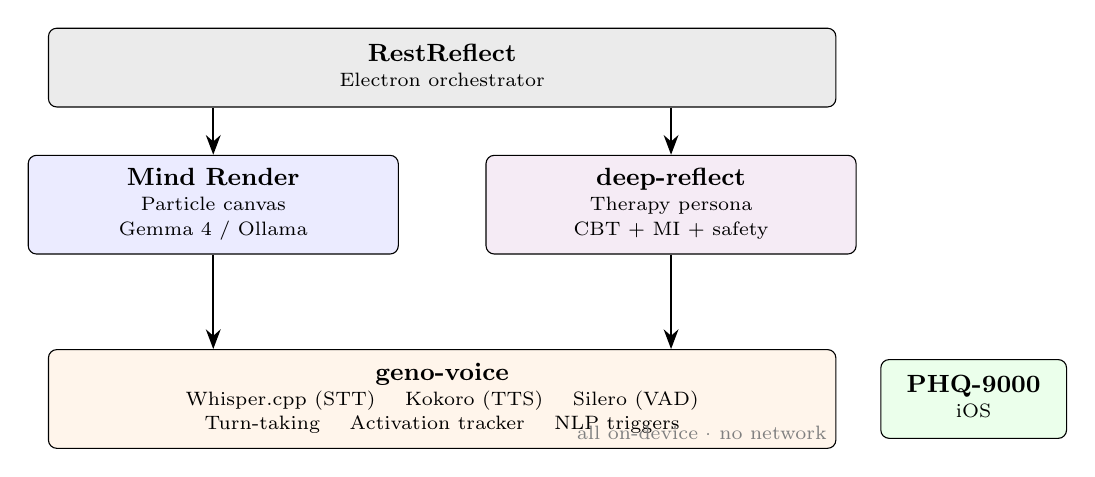
\begin{tikzpicture}[
    node distance=0.6cm and 0.4cm,
    box/.style={draw, rounded corners=3pt, minimum height=1cm, text centered, font=\small},
    wide/.style={box, minimum width=10cm},
    mid/.style={box, minimum width=4.7cm},
    label/.style={font=\scriptsize\color{gray}},
    arr/.style={-{Stealth[length=2.5mm]}, thick}
]

% Top layer
\node[wide, fill=black!8] (rest) {
    \begin{tabular}{c}
    \textbf{RestReflect} \\[-2pt]
    {\scriptsize Electron orchestrator}
    \end{tabular}
};

% Middle layer
\node[mid, fill=blue!8, below left=of rest.south, anchor=north east, xshift=-.15cm] (mind) {
    \begin{tabular}{c}
    \textbf{Mind Render} \\[-2pt]
    {\scriptsize Particle canvas} \\[-2pt]
    {\scriptsize Gemma 4 / Ollama}
    \end{tabular}
};

\node[mid, fill=violet!8, below right=of rest.south, anchor=north west, xshift=.15cm] (deep) {
    \begin{tabular}{c}
    \textbf{deep-reflect} \\[-2pt]
    {\scriptsize Therapy persona} \\[-2pt]
    {\scriptsize CBT + MI + safety}
    \end{tabular}
};

% Bottom layer
\node[wide, fill=orange!8, below=1.2cm of rest.south |- mind.south] (voice) {
    \begin{tabular}{c}
    \textbf{geno-voice} \\[-2pt]
    {\scriptsize Whisper.cpp (STT) \quad Kokoro (TTS) \quad Silero (VAD)} \\[-2pt]
    {\scriptsize Turn-taking \quad Activation tracker \quad NLP triggers}
    \end{tabular}
};

% PHQ-9000 side
\node[box, fill=green!8, minimum width=2cm, right=0.3cm of deep.east |- voice, anchor=west] (phq) {
    \begin{tabular}{c}
    \textbf{PHQ-9000} \\[-2pt]
    {\scriptsize iOS}
    \end{tabular}
};

% Arrows
\draw[arr] (rest.south -| mind.north) -- (mind.north);
\draw[arr] (rest.south -| deep.north) -- (deep.north);
\draw[arr] (mind.south) -- (mind.south |- voice.north);
\draw[arr] (deep.south) -- (deep.south |- voice.north);

% Local badge
\node[label, anchor=south east] at (voice.south east) {all on-device · no network};

\end{tikzpicture}
\caption{Component architecture. All components run on-device with no network dependencies.}
\label{fig:arch}
\end{figure}

\begin{table}[h]
\centering
\small
\caption{System components and their roles.}
\begin{tabular}{@{}lll@{}}
\toprule
Component & Role & Technology \\
\midrule
RestReflect & Orchestrator & Electron, Node.js \\
Mind Render & Visual canvas + LLM interface & Particle engine, Ollama \\
deep-reflect & Therapeutic persona + safety & System prompt, guardrails \\
geno-voice & Voice pipeline & Whisper.cpp, Kokoro, Silero \\
PHQ-9000 & Self-assessment & PHQ-9 instrument (iOS) \\
\bottomrule
\end{tabular}
\end{table}

\subsection{Model Selection}

RestReflect uses Gemma~4 (e4b variant, 4B active parameters via mixture-of-experts) running locally via Ollama with Metal backend on Apple Silicon. Selection criteria: open weights (auditable, fine-tunable), local execution on consumer hardware, and conversational quality sufficient for nuanced therapeutic dialogue. Fine-tuning uses Unsloth with LoRA on curated therapeutic dialogue datasets, with constitutional AI objectives to internalize safety in model weights.

\subsection{Voice Pipeline}

The pipeline is voice-first---typing disrupts reflective flow, and spoken interaction lowers the barrier to expression. Components: Whisper.cpp with Metal acceleration (STT), Kokoro synthesis (TTS), and Silero VAD for speech detection. The full pipeline runs with WiFi off.

%----------------------------------------------------------------------
\section{Therapeutic Design}
%----------------------------------------------------------------------

\subsection{Clinical Framework}

The persona implements Motivational Interviewing~\citep{miller2013motivational}---reflective listening, open-ended questions, affirming autonomy---and Cognitive Behavioral Therapy---identifying cognitive distortions, guided reframing. The system prompt instructs: ``Paraphrase what you hear before responding. Make the user feel heard before anything else.'' The persona never diagnoses, prescribes, or replaces professional care.

\subsection{Silence as Design}

In every mainstream voice agent, silence is a failure state. RestReflect inverts this: silence is the system's primary therapeutic tool. The turn-taking engine returns \textsc{stay\_silent} unless positive evidence---across multiple independent signals---says otherwise.

\paragraph{Adaptive silence windows.} Thresholds expand based on detected emotional state (Table~\ref{tab:silence}).

\begin{table}[h]
\centering
\small
\caption{Adaptive silence thresholds. Standard voice agents use 0.3--0.5\,s.}
\label{tab:silence}
\begin{tabular}{@{}lcc@{}}
\toprule
Condition & Backchannel (s) & Response (s) \\
\midrule
Baseline & 4.0 & 6.0 \\
Emotional content & 7.0 & 9.0 \\
User crying & 14.0 & 16.0 \\
Early session (first 2\,min) & 6.0 & 8.0 \\
\bottomrule
\end{tabular}
\end{table}

\paragraph{Multi-signal turn-taking.} The engine fuses four signals in a tiered architecture (Table~\ref{tab:signals}).

\begin{table}[h]
\centering
\small
\caption{Turn-taking signal hierarchy.}
\label{tab:signals}
\begin{tabular}{@{}llll@{}}
\toprule
Tier & Signal & Latency & Detects \\
\midrule
0 & Adaptive silence & real-time & Pause duration + emotional extension \\
1 & Smart Turn v2 & $\sim$50\,ms & Intonation, pace, filler words \\
2 & NLP triggers (regex) & $<$1\,ms & 30+ patterns: invitations, resignation \\
3 & LLM assessment & $\sim$500\,ms & Semantic analysis of ambiguous moments \\
\bottomrule
\end{tabular}
\end{table}

The fastest confident signal wins. ``I don't know anymore\ldots'' triggers the resignation pattern instantly via regex. A pause after a monologue needs Smart Turn to distinguish thinking from done. Ambiguous cases escalate to background LLM assessment.

\paragraph{The thinking-vs-waiting problem.} When the user is quiet, are they thinking (hold space) or waiting (respond)? A human therapist reads body language. RestReflect has only audio features and transcript history. The system errs on silence---interrupting processing is worse than making someone wait---with a 45-second gentle prompt as safety net. The visual state machine (Section~\ref{sec:vsm}) provides a complementary visual solution.

\subsection{Reflect Mode: The Core Interaction}

Reflect Mode is RestReflect's defining feature and the primary mode of interaction. Rather than answering the user, the system \emph{mirrors back what they said}---paraphrasing their words, naming their themes, and reflecting their emotional tone---before offering any response of its own. This implements the clinical technique of reflective listening~\citep{rogers1957necessary, miller2013motivational}, which serves three therapeutic functions: \emph{validation} (the speaker feels heard, reducing defensiveness), \emph{cognitive reprocessing} (hearing one's own thoughts externalized enables evaluation and refinement), and \emph{ambivalence exploration} (reflections surface contradictions the speaker may not have noticed).

\citet{magill2018meta} found that therapist reflective listening correlated with client change talk at $r = .55$ ($p < .001$), with complex reflections---those that infer meaning beyond what was literally said---predicting the highest rates of change talk. \citet{kumar2024gpt4} demonstrated that LLMs can generate such complex reflections with 88\% clinician-rated acceptability. Reflect Mode operationalizes these findings in a real-time voice pipeline.

\paragraph{The reflect pipeline.} Three processes run concurrently:

\begin{enumerate}
\item \textbf{Live transcription.} Whisper.cpp streams STT chunks while the user speaks, producing running text that feeds downstream analysis.
\item \textbf{Concurrent LLM analysis.} Via Pipecat's \texttt{ParallelPipeline}, Gemma~4 processes transcript chunks in the background---identifying emotional content, extracting themes, and preparing reflective material---while the user is still speaking.
\item \textbf{Reflection synthesis.} When the turn-taking engine signals that a response is warranted, the LLM generates a reflective restatement (not an answer), and Kokoro synthesizes it as speech.
\end{enumerate}

The system is selective about \emph{when} to reflect---silence is the default (Section~4.2)---but once the turn-taking engine commits to a response, time to first speech is critical. In therapeutic conversation, the moment after someone shares something vulnerable is when silence shifts from ``holding space'' to ``feeling dismissed.'' The latency budget from decision-to-speak to first audible sound must stay within $\sim$1--2\,s.

\paragraph{Transcription reliability.} Whisper produces hallucinations in always-listening mode---``Thanks for watching,'' ``[music],'' repetitive loops---because silence and ambient noise are frequent in therapeutic sessions. A dedicated filter uses 8~regex patterns for common Whisper artifacts, filler-only detection, and a repetitiveness check (discard when unique words $< 30$\% of total). NLP trigger patterns were calibrated against 279~diarized examples from 6~episodes of real therapy podcasts.

\paragraph{Simple vs.\ complex reflections.} The persona prompt guides Gemma~4 toward complex reflections---inferring unstated meaning, naming emotions the user danced around, connecting themes across the session---rather than simple restatements. After a user says ``I keep trying to make it work but nothing changes,'' a simple reflection would be ``It sounds like nothing is changing despite your efforts.'' A complex reflection might be: ``There's a part of you that hasn't given up, even though it's exhausting.'' The latter validates the effort, names the exhaustion, and surfaces the persistence the user didn't explicitly claim---all without offering advice.

\subsection{Optimizing the Response Path}

Once the system decides to speak, multiple architectural choices minimize time to first speech:

\paragraph{Precomputed acknowledgments.} 63~WAV clips across 7~cue types (``I hear you,'' ``Go on,'' ``That sounds difficult'') $\times$ 3~variants $\times$ 3~voices are pre-synthesized at startup. When TTS latency for the full reflection would exceed the comfort threshold, a precomputed clip plays immediately---the user hears something within hundreds of milliseconds while the real response streams behind it.

\paragraph{Parallel pipeline.} Pipecat's \texttt{ParallelPipeline} enables background LLM processing while the user is still speaking. Session note analysis, theme extraction, and response planning happen concurrently with STT, so when the turn-taking engine signals \textsc{speak}, the LLM has already been primed with context.

\paragraph{Tiered signal speed.} The turn-taking engine's tiered architecture doubles as a latency optimization. NLP triggers fire in $<$1\,ms---if the user says ``what do you think?'' the system can begin generating a response immediately, before the 50\,ms Smart Turn score or 500\,ms LLM assessment arrive. The fastest confident signal starts the response pipeline.

\paragraph{Visual latency masking.} The big crunch animation (Section~\ref{sec:vsm}) serves a dual purpose: it communicates ``the system is preparing a response'' while buying time for LLM inference and TTS synthesis. The user perceives intentional processing rather than dead latency, fundamentally changing the experience of a 2--3\,s generation delay.

\paragraph{Single model instance.} Using Gemma~4 e4b for both conversational response and background session analysis avoids GPU context-switching overhead on Apple Silicon's unified memory, keeping the response path fast when it matters.

\subsection{Visual State Machine}
\label{sec:vsm}

The particle canvas communicates system state without breaking silence---the digital equivalent of a therapist's body language. Three states:

\begin{enumerate}
\item \textbf{Listening (ambient float).} 2200 particles drift in Lissajous patterns, modulated by the activation tracker. Communicates presence without speaking.
\item \textbf{Responding (spectrum disturbance).} TTS audio routed through a Web Audio \texttt{AnalyserNode}. Frequency bands map to particle displacement vectors---the ambient float is \emph{disturbed} by the agent's voice, settling back when speech ends.
\item \textbf{Deep reflect (big crunch).} All particles collapse to a singularity (reverse big bang), signaling concentration. When the reflection is ready, a new big bang explodes outward.
\end{enumerate}

State transitions (Figure~\ref{fig:vsm}) are read peripherally. A shift from floating to collapsing registers as ``something is happening'' without requiring sound.

\begin{figure}[h]
\centering
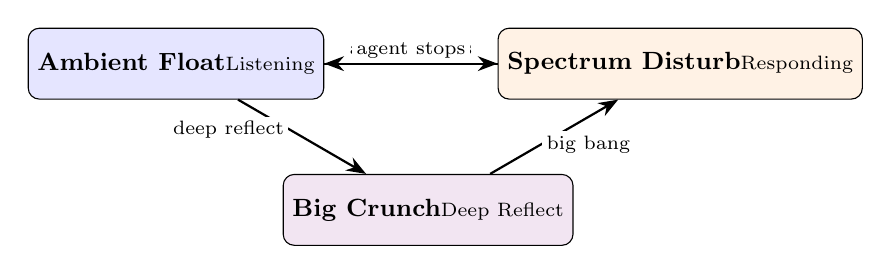
\begin{tikzpicture}[
    node distance=2.2cm,
    state/.style={draw, rounded corners=4pt, minimum width=2.6cm, minimum height=0.9cm, text centered, font=\small},
    arr/.style={-{Stealth[length=2.5mm]}, thick},
    lbl/.style={font=\scriptsize, midway, fill=white, inner sep=1.5pt}
]

\node[state, fill=blue!10] (listen) {\textbf{Ambient Float}\\[-2pt]{\scriptsize Listening}};
\node[state, fill=orange!10, right=of listen] (respond) {\textbf{Spectrum Disturb}\\[-2pt]{\scriptsize Responding}};
\node[state, fill=violet!10, below=1.4cm of $(listen)!0.5!(respond)$] (crunch) {\textbf{Big Crunch}\\[-2pt]{\scriptsize Deep Reflect}};

\draw[arr] (listen) -- node[lbl, above] {agent speaks} (respond);
\draw[arr] (respond) -- node[lbl, above] {agent stops} (listen);
\draw[arr] (listen) -- node[lbl, left, pos=0.4] {deep reflect} (crunch);
\draw[arr] (crunch) -- node[lbl, right, pos=0.4] {big bang} (respond);

\end{tikzpicture}
\caption{Visual state machine. The particle canvas transitions between three states to communicate system behavior without audio.}
\label{fig:vsm}
\end{figure}

\subsection{Emotion Wheel}

When the user struggles to name their feeling (detected via NLP patterns), particles rearrange into \citet{plutchik1980general}'s emotion wheel---8~petals $\times$ 3~intensity rings, rotatable via scroll. This implements affect labeling~\citep{lieberman2007putting} as a purely visual+gestural interaction. Selection feeds the named emotion to the LLM as context.

\subsection{Emotional Activation Tracking}

Real-time emotional state from raw audio, no ML dependencies: pitch (F0 via autocorrelation), energy (RMS), vocal tension (ZCR), energy variance. Features z-scored against a per-session speaker baseline (first 5~chunks), fused as $0.30 \cdot \text{RMS} + 0.25 \cdot F0 + 0.25 \cdot F0_\text{var} + 0.10 \cdot \text{ZCR} + 0.10 \cdot E_\text{var}$, passed through a sigmoid. Dual-rate EMA (fast $\alpha = 0.3$, slow $\alpha = 0.05$) tracks trajectory. Feeds turn-taking (threshold extension), the visual canvas (particle turbulence), and crying detection.

%----------------------------------------------------------------------
\section{Privacy and Safety}
%----------------------------------------------------------------------

\paragraph{Privacy by design.} Privacy is architectural: no network calls, no telemetry, no cloud fallback. The app works offline. The population most in need---those dealing with trauma, shame, or stigma---is least likely to trust cloud services. Local-only removes the trust barrier entirely.

\subsection{Data Transparency and User Control}

Privacy by design means the data stays local---but ``local'' is not the same as ``understood.'' Users must know exactly what is stored, where it lives, and how to control it. RestReflect makes this explicit through three mechanisms.

\paragraph{Visible file paths.} All session artifacts---audio recordings, transcripts, session notes, PHQ-9 scores, activation logs---are stored in a user-visible directory under the platform's standard application data path (\texttt{\char`\~/Library/Application Support/mind-render/} on macOS). The app surfaces these paths in a data management panel, not buried in documentation. Each session shows its folder path, file sizes, and creation date.

\paragraph{Granular deletion.} Users can delete individual sessions or all data via a single action in the app. Deletion is immediate and unrecoverable---no soft-delete, no trash, no ``are you sure you want to permanently delete'' dark pattern that discourages exercising the right. The system also supports session-level recording opt-out: users can disable audio recording for a session while keeping transcription active, or disable all persistence entirely for a fully ephemeral conversation.

\paragraph{Export and secure storage.} Sessions can be exported to an encrypted archive for backup or transfer to another device. First-launch onboarding walks users through what will be stored, where, and how to control it---establishing informed consent before the first therapeutic interaction, not after.

This transparency serves a therapeutic function beyond compliance. When users can see that their session recording is a WAV file in a folder they control---not a row in a database they cannot access---the privacy guarantee becomes tangible. Trust is built from evidence, not promises.

\subsection{Safety and Resource Referral}

Safety in RestReflect operates at three levels: crisis intervention, proactive human connection, and contextual resource referral.

\paragraph{Crisis detection.} PHQ-9~\citep{kroenke2001phq9} item~9 screens suicidal ideation, triggering an immediate crisis protocol: compassionate acknowledgment, 988~Suicide \& Crisis Lifeline referral, and a grounding exercise. Keyword and semantic detection for self-harm and harm to others provides a second layer. Constitutional AI fine-tuning objectives internalize safety in model weights beyond system prompts---safety should survive prompt injection.

\paragraph{Encouraging human connection.} A reflection tool that becomes someone's only outlet has failed. The deep-reflect persona is prompted to proactively encourage users toward real human relationships---suggesting they talk to a friend, reach out to a family member, or reconnect with someone they trust. This is not a disclaimer appended to responses but a therapeutic stance woven into the persona: the system models the belief that human connection is more healing than any AI interaction. When a user describes isolation, the system reflects on it \emph{and} gently explores what outreach might look like.

\paragraph{Program-aware reflections.} When conversation content aligns with established recovery and support programs, the system incorporates their principles with proper attribution. A user processing substance dependence may hear reflections that draw on the twelve-step tradition's concept of powerlessness and surrender---not as prescription, but as a framework for the user to examine. Similarly, discussions of codependency, compulsive behavior, grief, or anger can surface principles from Al-Anon, SMART Recovery, SLAA, or grief support frameworks. The persona references these as ``some people find it helpful to\ldots'' rather than directing the user, preserving autonomy.

\paragraph{Local resource database.} The system maintains an on-device database of actionable resources:

\begin{itemize}
\item \textbf{Meeting directories} --- US locations for 12-step and recovery programs (AA, NA, Al-Anon, SLAA, SMART Recovery), searchable by zip code or city.
\item \textbf{Affordable therapy} --- sliding-scale therapy directories, community mental health centers, university training clinics, and online options (Open Path Collective, BetterHelp financial aid).
\item \textbf{Crisis lines} --- 988 Lifeline, Crisis Text Line, Trevor Project, Veterans Crisis Line, and specialized hotlines.
\item \textbf{Support communities} --- NAMI support groups, peer support networks, and condition-specific organizations.
\end{itemize}

Resources surface contextually---when the conversation naturally reaches a point where a referral would be helpful---not as a list dump. The database ships with the app and updates via optional periodic syncs, keeping the local-first guarantee intact for offline use.

\paragraph{PHQ-9 integration.} PHQ-9000 implements the Patient Health Questionnaire-9~\citep{kroenke2001phq9} as a local iOS companion. Optional session-close check-in with longitudinal score tracking. Rising scores trigger the persona to more actively encourage professional consultation and surface affordable therapy resources. All scores stored locally.

%----------------------------------------------------------------------
\section{Technical Challenges}
%----------------------------------------------------------------------

\paragraph{Native audio inference.} Gemma~4 e4b accepts audio natively, preserving paralinguistic cues. Ollama's Go-native sampler silently ignores \texttt{repeat\_penalty}, \texttt{frequency\_penalty}, and \texttt{presence\_penalty}---producing 84.7\% WER on 25-second passages from repetition loops. We implemented the missing penalties (224~lines, 6~files) matching llama.cpp's algorithm (PR~\#15784). Performance remains too slow for real-time; current approach: Whisper for live conversation, native audio for post-session analysis.

\paragraph{GPU contention.} Running Whisper + Gemma~4 + Kokoro concurrently on a single Apple Silicon GPU creates contention. Using one model instance for both chat and session analysis avoids context-switching overhead.

\paragraph{Backchannel failure.} Automated backchannel signals fired at wrong times---mid-sentence, on ambient noise, during contemplative silences. The core issue: distinguishing ``pause within a thought'' from ``pause inviting acknowledgment'' requires pragmatic understanding that VAD thresholds cannot provide. Shelved in favor of precomputed acknowledgments.

%----------------------------------------------------------------------
\section{Evaluation Framework}
%----------------------------------------------------------------------

We propose evaluation across six dimensions: (1)~therapeutic quality via expert transcript review against CBT/MI criteria; (2)~safety via red-team testing of crisis detection; (3)~privacy via network traffic analysis confirming zero outbound connections; (4)~voice quality via latency benchmarks and TTS naturalness ratings; (5)~user experience via qualitative assessment of trust and canvas utility; and (6)~clinical outcome via longitudinal PHQ-9 trajectories (requiring IRB-approved pilot).

%----------------------------------------------------------------------
\section{Limitations}
%----------------------------------------------------------------------

Hardware requirements (16--32\,GB RAM) limit accessibility. Local model quality lags frontier cloud models. No clinical validation via controlled trials. CBT and MI are Western-centric frameworks. The system cannot handle severe mental illness beyond crisis routing. Local models may be more susceptible to jailbreaking than API-guarded models.

Future directions include clinical pilot studies with IRB approval, per-user silence adaptation across sessions, multimodal input (camera-based body language with consent), expanded modalities (DBT, ACT), and smaller models for broader accessibility.

%----------------------------------------------------------------------
\section{Conclusion}
%----------------------------------------------------------------------

RestReflect demonstrates that a therapeutic voice companion can be built on fundamentally different assumptions than mainstream voice agents. Where standard agents optimize response speed indiscriminately, RestReflect is strategic about \emph{when} to speak and aggressive about \emph{how fast} to speak once committed. Where standard agents send audio to the cloud, RestReflect keeps everything local. Where standard agents treat silence as dead time, RestReflect treats it as the primary therapeutic tool---while ensuring that time to first speech, when a response is warranted, remains optimized through parallel processing, precomputed acknowledgments, and visual latency masking.

The system is not a replacement for human therapy. It is a reflection tool for the space between sessions, for the things too raw to say to another person, and for the many people who will never access professional care. By solving the privacy problem architecturally rather than contractually, RestReflect removes the trust barrier that prevents the most vulnerable users from engaging with AI-assisted mental health support.

%----------------------------------------------------------------------
\bibliographystyle{plainnat}
\bibliography{references}

\end{document}
